
\chapter{Conception}

Lors de chapitre on va s'immerger de plus en lus dans les d\'{e}tails de la conception ,
on va tout d'abord illustrer les diagrammes de cas d'utilisation et par la suite nous définissons le product backlog etla planification des sprints,puis on va illustrer les diagrammes de s'{e}quences et le diagramme de classes en donnant une description d\'{e}taill\'{e} à notre base de donn\'{e}es.
Et nous finissons par  une description plus d\'{e}taill\'{e} en passant par les diagrammes d'activit\'{e} et de d\'{e}ploiement.


\section{Diagrammes de cas d'utilisation}




\subsection{ Diagrammes de cas d'utilisation d\'{e}taill\'{e}s }


Dans cette partie, nous allons raffiner les cas d’utilisation prioritaires et les
décrire en détail afin de mieux visualiser notre application.



\subsubsection{ Diagramme de cas d'utilisation "G\'{e}rer un projet"}
D\'{e}tailler le cas d'utilisation \guillemotleft{}G\'{e}rer un projet \guillemotright{} revient \`{a} d\'{e}tailler son propre
cas d'utilisation ainsi que ses 4 sous cas d'utilisation \`{a} savoir :

\begin{itemize}
\item{ G\'{e}rer un projet.}
\item{ G\'{e}rer  un membre.}
\item{ G\'{e}rer un client.}
\item{ G\'{e}rer  une t\^{a}che.}
\end{itemize}

\subsubsection{ Diagramme de cas d'utilisation "G\'{e}rer un projet"}

\begin{figure}[H]
\center
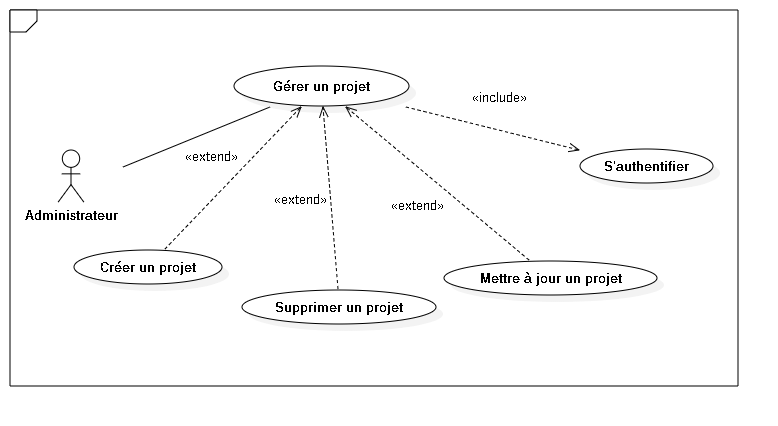
\includegraphics[width=13cm,height=8cm]{./figures/ucP.png}
\caption{G\'{e}rer un projet.}

\end{figure}



\subsubsection{ Diagramme de cas d'utilisation "G\'{e}rer un membre"}
\begin{figure}[H]
\center
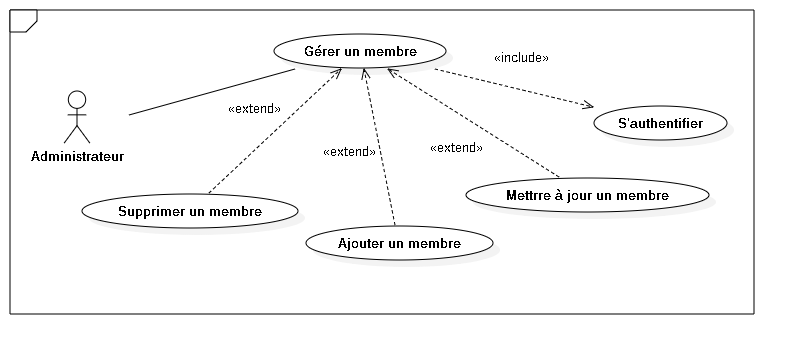
\includegraphics[width=13cm,height=8cm]{./figures/ucM.png}
\caption{G\'{e}rer un membre.}

\end{figure}


\subsubsection{ Diagramme de cas d'utilisation "G\'{e}rer un client"}
\begin{figure}[H]
\center
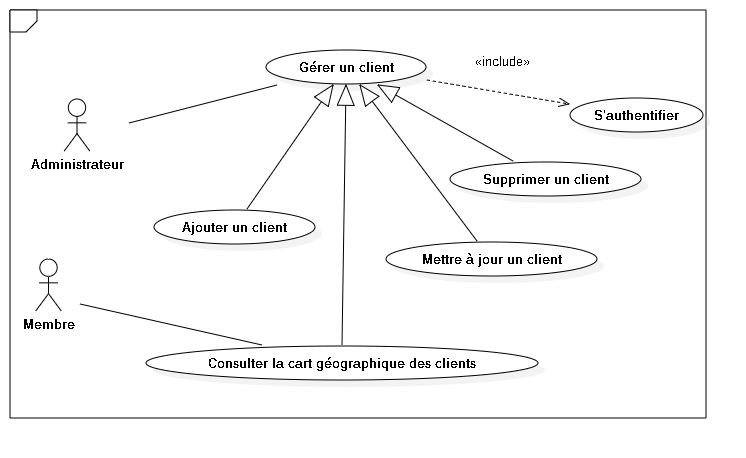
\includegraphics[width=13cm,height=8cm]{./figures/ucC.png}
\caption{G\'{e}rer un client.}
\end{figure}

\subsubsection{ Diagramme de cas d'utilisation "G\'{e}rer une t\^{a}che"}
\begin{figure}[H]
\center
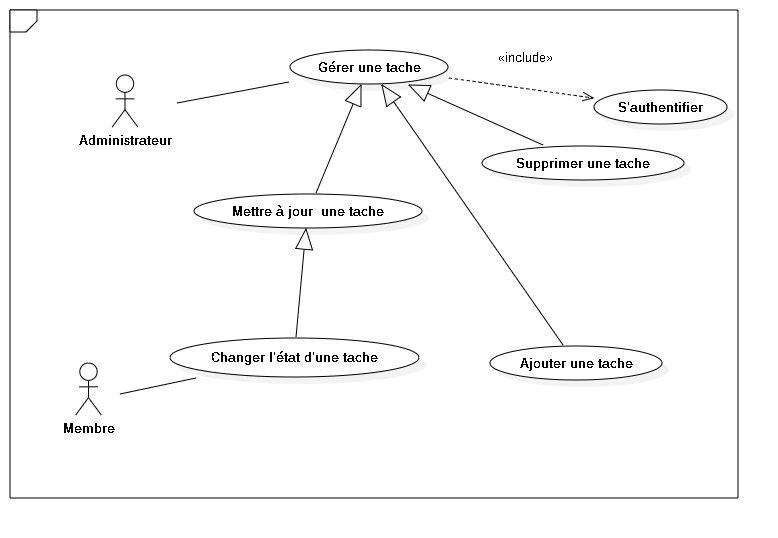
\includegraphics[width=13cm,height=8cm]{./figures/ucT.png}
\caption{G\'{e}rer une t\^{a}che.}

\end{figure}







\section{Backlog de planning}


Apr\'{e}s avoir d\'{e}finit les acteurs des systémes et les diff\'{e}rentes interactions nous pouvons maintenant définir notre Product Backlog
puis nous pr\'{e}cisions la planification des sprints.

\subsection{Les fonctionnalit\'{e}s du Backlog}
Le Backlog est un art\'{e}fact tr\`{e}s important dans SCRUM. C'est l'ensemble des caract\'{e}ristiques
fonctionnelles ou techniques qui constituent le produit souhait\'{e}.
Nous allons les d\'{e}crire en d\'{e}tails dans le tableau qui suit :



\begin{table}

\begin{tabular}{|l|l|l|}
\hline
Fonctionnalité                                                                                              & Acteur                          & Description                                                                                                                                                     \\
\hline
Gérer un projet                                                                                             & Administrateur                  & \begin{tabular}[c]{@{}l@{}}L’administrateur peut gérer un projet et ses \\tâches correspondantes d’affectation\end{tabular}                                     \\
\hline
Mettre à jour un                                                                                            & \multirow{3}{*}{Administrateur} & \multirow{3}{*}{\begin{tabular}[c]{@{}l@{}}L’administrateur peut changer les détails \\du projet ainsi que l’affectation des membres\\~au projet\end{tabular}}  \\
\cline{1-1}
Projet                                                                                                      &                                 &                                                                                                                                                                 \\
\cline{1-1}
                                                                                                            &                                 &                                                                                                                                                                 \\
\hline
\begin{tabular}[c]{@{}l@{}}Créer ,Modifier ,\\Supprimer un membre\end{tabular}                              & Administrateur                  & \begin{tabular}[c]{@{}l@{}}L’administrateur peut manipuler les données \\des membres\end{tabular}                                                               \\
\hline
\begin{tabular}[c]{@{}l@{}}Créer ,Modifier ,\\Supprimer un client\end{tabular}                              & Administrateur                  & \begin{tabular}[c]{@{}l@{}}L’administrateur peut manipuler les \\données des clients\end{tabular}                                                               \\
\hline
Consulter les rapports                                                                                      & Administrateur                  & L’administrateur peut accéder aux rapports                                                                                                                      \\
\hline
\begin{tabular}[c]{@{}l@{}}Consulter les coordonnées \\des clients sur la carte\\~géographique\end{tabular} & Administrateur                  & \begin{tabular}[c]{@{}l@{}}L’administrateur peut accéder aux \\coordonnées géographiques des clients\end{tabular}                                               \\
\hline
\begin{tabular}[c]{@{}l@{}}Changer l’état et la\\~progression approximative \\de ses tâches\end{tabular}    & Membre                          & \begin{tabular}[c]{@{}l@{}}Le membre peut changer ses taches \\courantes selon l’avancement.\end{tabular}                                                       \\
\hline
\end{tabular}
\centering
\caption{Product Backlog}
\end{table}

\newpage

\subsection{ Planification des sprints}

\FloatBarrier
\begin{table}

\begin{tabular}{|l|l|l|}
\hline
\multirow{2}{*}{Release 1} & Gestion des projets                        & 20 jours  \\
\cline{2-3}
                           & Gestion des membres                        & 7 jours   \\
\hline
\multirow{5}{*}{Release 2} & Gestion des clients                        & 2 jours   \\
\cline{2-3}
                           & Authentification                           & 5 jours   \\
\cline{2-3}
                           & Création des interfaces administrateurs    & 20 jours  \\
\cline{2-3}
                           & Création des interfaces membres            & 5 jours   \\
\cline{2-3}
                           & Modification et design des interfaces~ ~ ~ & 15 jours  \\
\hline
\multirow{2}{*}{Release 3} & Intégration des données                    & 10 jours  \\
\cline{2-3}
                           & Affichage des rapports                     & 7 jours   \\
\hline

\end{tabular}
\centering
\caption{Planification des sprints }
\end{table}
\FloatBarrier


\subsection{Diagramme de Gantt}

\FloatBarrier
\begin{figure}[H]
\center
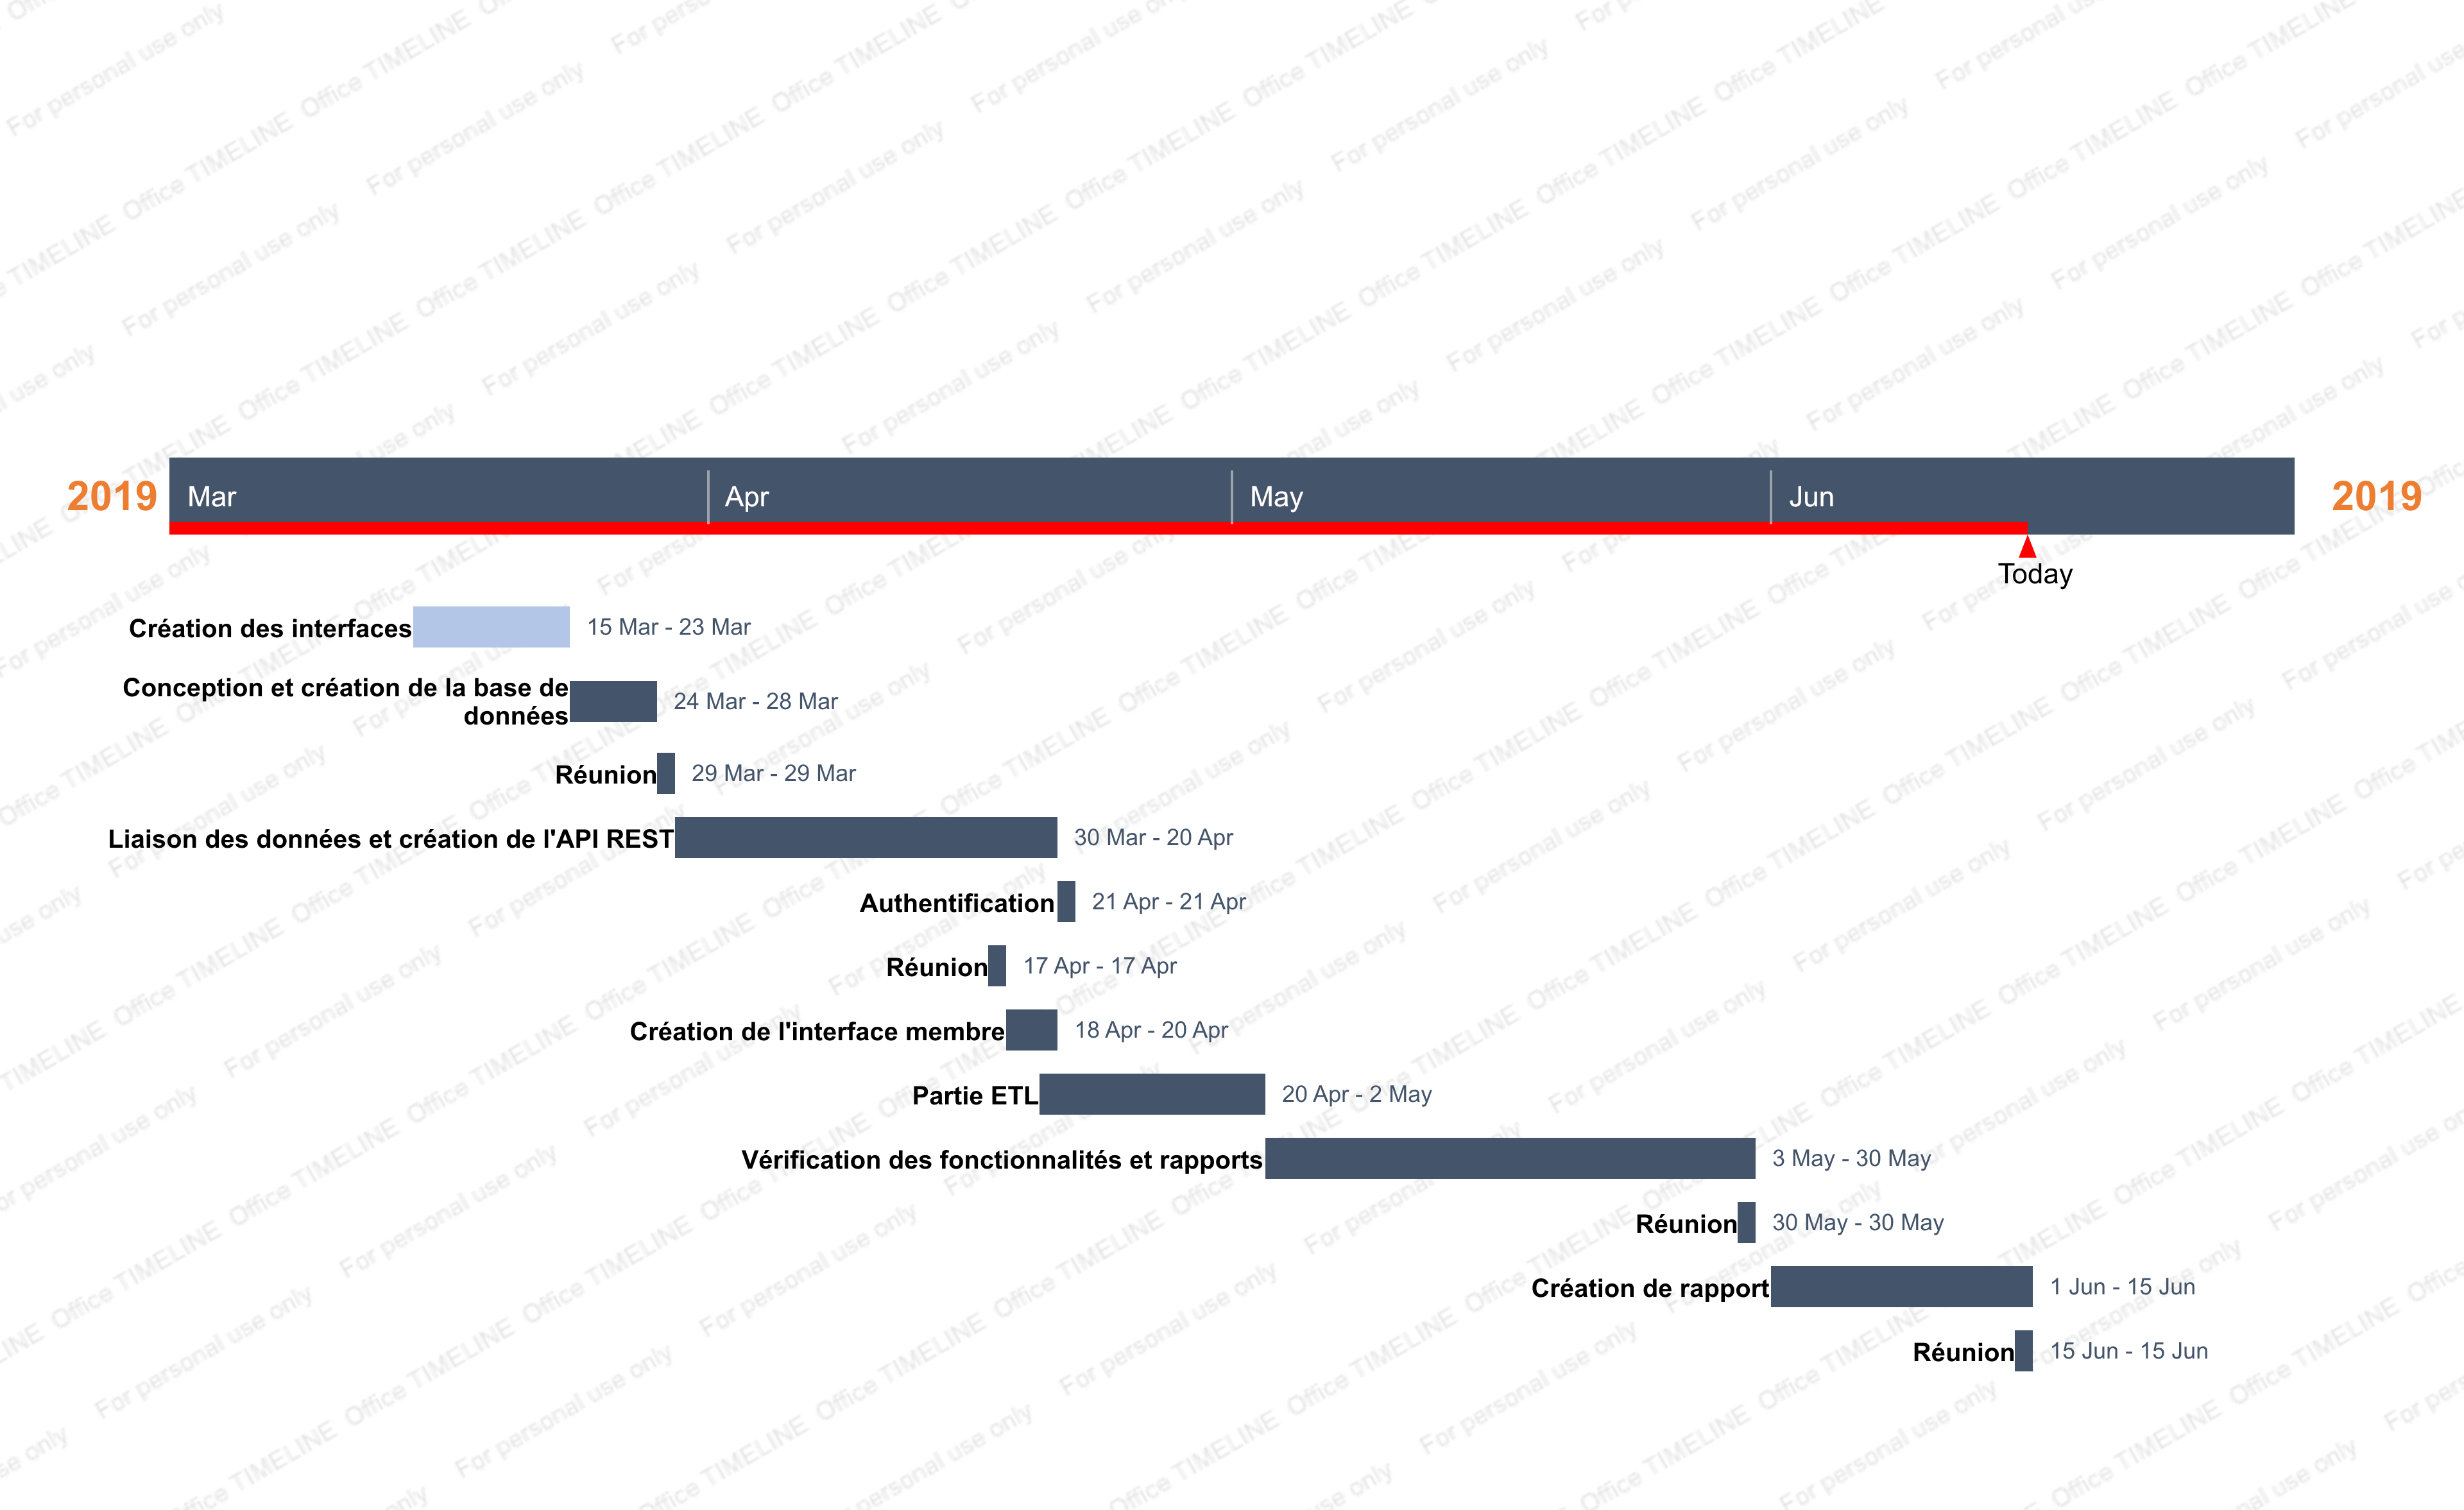
\includegraphics[width=15cm,height=15cm]{./figures/gantt.png}
\caption{Diagramme de Gantt.}
\end {figure}
\FloatBarrier


\FloatBarrier

\section{Diagrammes de séquences}



%interface membre


\newpage

\subsubsection{Le sc\'{e}nario \guillemotleft{} Consultation des rapports\guillemotright{}}
Le diagramme de s\'{e}quence \guillemotleft{} Ajout d'une t\^{a}che \guillemotright{} pr\'{e}sente le s\'{e}quencement
des interactions entre Administrateur, Application et Base de donn\'{e}es (BD).


\begin{figure}[H]
\center
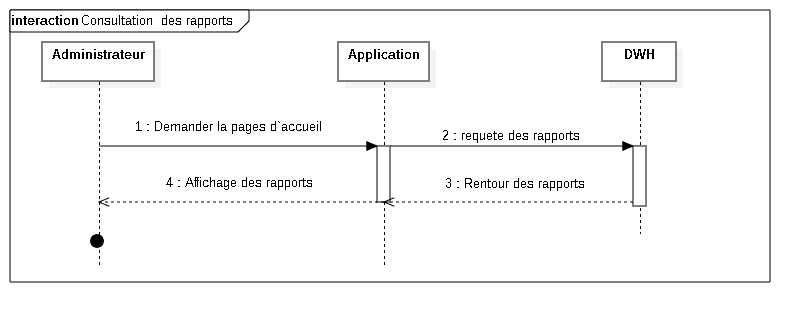
\includegraphics[width=14cm,height=9cm]{./figures/seq/G.png}
\caption{Consultation des rapports.}
\end{figure}



\begin{figure}[H]
\center
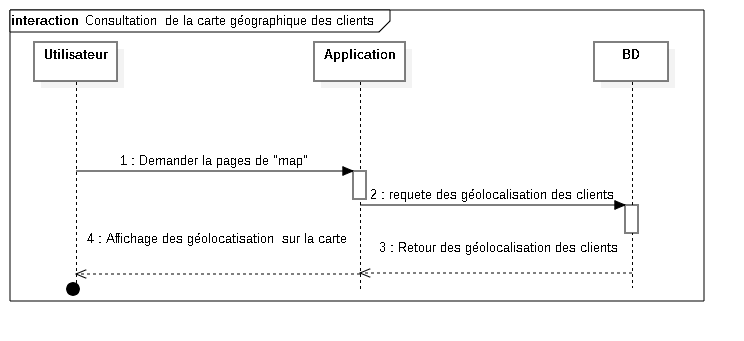
\includegraphics[width=14cm,height=8cm]{./figures/seq/H.png}
\caption{Consultation de la carte g\'{e}ographique des clients.}
\end{figure}
\newpage





\section{Diagramme de classes }



\section{Conception de la base de donn\'{e}es}

\subsection{Mod\`{e}le du liason des donn\'{e}es }
L'architecture de notre application nous implique \`{a} cr\'{e}er un mod\`{e}le physique
des donn\'{e}es , et nous avons pas \'{e}t\'{e} besoin d'un model conceptuel logique
,puisque on a li\'{e}e directement les donn\'{e}es \`{a} l'application par le biais d'un
pilote de connexion et pas par un ORM , et ceci est le diagramme
Entit\'{e}s \textendash{}Relations de la base de donn\'{e}es qui est en interaction avec
l'application web .
Choix de la m\'{e}thodologie de conception :
La liaison par des ORM ,ou poss\'{e}de des avantages bienque des inconv\'{e}nient ,
parmi ses avantages :

\bigskip
\begin{itemize}
\item{\textbf{La portabilit\'{e} :}  ORM est utilis\'{e} pour que vous \'{e}criviez votre structure une
seule fois et la couche ORM g\'{e}rera l'instruction finale adapt\'{e}e au SGBD
configur\'{e}. C'est un excellent avantage, car une op\'{e}ration simple, telle que
limit, est ajout\'{e}e sous la forme "limit 0,100" \`{a} la fin de l'instruction select
dans MySQL, alors qu'elle est "select top 100 from table" dans MS SQL.}

\bigskip
\item{\textbf{Imbrication de donn\'{e}es:} en cas de relations, la couche ORM extraira
automatiquement les donn\'{e}es pour vous.}

\bigskip
\item{\textbf{Langage unique:} vous ne connaissez pas le langage SQL pour traiter la base
de donn\'{e}es uniquement avec votre langage de d\'{e}veloppement.
Ajouter revient \`{a} modifier: la plupart des couches ORM traitent l'ajout de
nouvelles donn\'{e}es (insertion SQL) et la mise \`{a} jour des donn\'{e}es (SQL
Update) de la m\^{e}me mani\`{e}re, ce qui facilite grandement l'\'{e}criture et la
maintenance du code.}

\item{\textbf{Imbrication de donn\'{e}es:} en cas de relations, la couche ORM extraira
automatiquement les donn\'{e}es pour vous.}

\end{itemize}

\bigskip

Et parmi les inconv\'{e}nients de l'ORM on trouve :



\bigskip

\begin{itemize}
\item{\textbf{ La complexit\'{e} des requ\^{e}tes : }certaines couches ORM ont des limitations, en
particulier lors de l'ex\'{e}cution de requ\^{e}tes. Vous serez donc parfois oblig\'{e}
d'\'{e}crire en SQL brut.}

\item{\textbf{Lenteur:}
 si vous comparez les performances entre l'\'{e}criture de SQL brut ou
l'utilisation d'ORM, vous trouverez le brut beaucoup plus rapidement car il
n'y a pas de couche de traduction.}

\item{\textbf{R\'{e}glage:} si vous connaissez bien le langage SQL et votre SGBD par d\'{e}faut,
vous pouvez utiliser vos connaissances pour acc\'{e}l\'{e}rer les requ\^{e}tes, mais ce
n'est pas la m\^{e}me chose avec ORM.}

\item{\textbf{Configuration:}
 si vous travaillez dans un projet Big Data et que vous n'\^{e}tes
pas satisfait de la performance, vous vous retrouverez en train d'\'{e}tudier la
couche ORM afin de pouvoir minimiser les occurrences du SGBD.}



\end{itemize}


\subsection{Diagramme de classes}

\begin{figure}[H]
\center
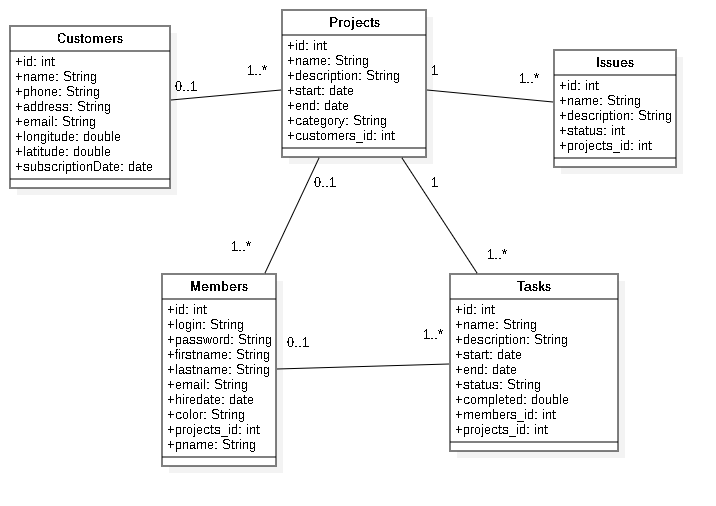
\includegraphics[width=13cm,height=11cm]{./figures/class.png}
\caption{Diagramme de classes.}

\end{figure}
\FloatBarrier

\subsubsection{Tableau explicatif}

Afin de clarifier ce sh\'{e}ma en explicant les diff\'{e}rents relations pour les
entit\'{e}s ,nous avons choisi de les mettre dans un tableau descriptif .
\FloatBarrier

\begin{table}

\begin{tabular}{|l|l|l|l|l|}
\hline
Nom relation                        & Entité E1                 & Entité E2                  & Relation(E1:E2) & Relation(E2:E1)  \\
\hline
\multirow{2}{*}{Projects -Tasks}    & \multirow{2}{*}{Projects} & \multirow{2}{*}{Tasks}     & 1 : N           & 1 : 1            \\
\cline{4-5}
                                    &                           &                            & Non-identifiée  & identifiée       \\
\hline
\multirow{2}{*}{Projects -Members}  & \multirow{2}{*}{Projects} & \multirow{2}{*}{Members}   & 1~: N           & 1~: 1            \\
\cline{4-5}
                                    &                           &                            & Non-identifiée  & Non-identifiée   \\
\hline
\multirow{2}{*}{Members-Tasks}      & \multirow{2}{*}{Members}  & \multirow{2}{*}{Tasks}     & 1~: N           & 1~: 1            \\
\cline{4-5}
                                    &                           &                            & Non-identifiée  & Non-identifiée   \\
\hline
\multirow{2}{*}{Projects-Customers} & \multirow{2}{*}{Projects} & \multirow{2}{*}{Customers} & 1~: 1           & 1~: N            \\
\cline{4-5}
                                    &                           &                            & Non-identifiée  & Non-identifiée   \\
\hline
\end{tabular}
\centering
\caption {Relations}

\end{table}

\FloatBarrier



Les relations peuvent etre expliqu\'{e}es par les r\'{e}gles suivantes:
\begin{itemize}
\item{ Une relation non identifi\'{e}e 1 :N  entre une entit\'{e} E1 et une autre E2:}
Pour E1 il existe ou il n'existe pas une ou plusieurs entit\'{e}s E2
\bigskip

\item{Une relation non identifi\'{e}e 1 :1 entre une entit\'{e} E1 et une autre E2:}
Pour E1 il existe ou il n'existe pas une entit\'{e} E2
\bigskip

\item{Une relation identifi\'{e}e 1 :N entre une entit\'{e} E1 et une autre E2: }
 Pour E1 il existe une ou plusieurs entit\'{e}s E2
 \bigskip

\item{Une relation identifi\'{e}e 1 :1 entre une entit\'{e} E1 et une autre E2: }
 Pour E1 il existe une entit\'{e} E2
 \bigskip

\end{itemize}

\newpage

\subsubsection{Description d\'{e}taill\'{e}e}
\bigskip
Ainsi nous avons utilis\'{e} la requite \textquotedblleft{}describe NOM\_TABLE\textquotedblright{} qui est
disponible dans le langage MySQL et qui permet de d\'{e}crir les champs ,leurs
types et leurs sp\'{e}cifications pour chaque table utilis\'{e}e
Ces figures montrent la description d\'{e}taill\'{e}e de chaque table utilis\'{e}e dans
notre application:
\bigskip

\begin{itemize}


\item{La table \guillemotleft{} projects \guillemotright{}}


\begin{table}

\begin{tabular}{|l|l|l|l|l|l|}
\hline
Field         & Type          & Null & Key & Default & Extra            \\
\hline
id            & int(11)       & NO   & PRI & NULL    & auto\_increment  \\
\hline
name          & varchar(45)   & NO   &     & NULL    &                  \\
\hline
description   & varchar(1000) & YES  &     & NULL    &                  \\
\hline
start         & date          & NO   &     & NULL    &                  \\
\hline
end           & date          & NO   &     & NULL    &                  \\
\hline
category      & varchar(60)   & YES  &     & NULL    &                  \\
\hline
customers\_id & int(11)       & YES  & MUL & NULL    &                  \\
\hline
\end{tabular}
\centering
 \caption {Projects.}
\end{table}


\item{La table \guillemotleft{} tasks \guillemotright{}}

\begin{table}

\begin{tabular}{|l|l|l|l|l|l|}
\hline
Field        & Type         & Null & Key & Default            & Extra            \\
\hline
id           & int(11)      & NO   & PRI & NULL               & auto\_increment  \\
\hline
login        & varchar(30)  & YES  &     & NULL               &                  \\
\hline
password     & varchar(15)  & YES  &     & NULL               &                  \\
\hline
firstname    & varchar(50)  & YES  &     & NULL               &                  \\
\hline
lastname     & varchar(30)  & YES  &     & NULL               &                  \\
\hline
email        & varchar(100) & YES  &     & NULL               &                  \\
\hline
hiredate     & datetime     & YES  &     & CURRENT\_TIMESTAMP &                  \\
\hline
color        & varchar(6)   & YES  &     & NULL               &                  \\
\hline
projects\_id & int(11)      & YES  & MUL & NULL               &                  \\
\hline
pname        & varchar(50)  & YES  &     & NULL               &                  \\
\hline
\end{tabular}
\centering
 \caption {Tasks.}
\end{table}




\item{La table \guillemotleft{} members \guillemotright{}}

\begin{table}

\begin{tabular}{|l|l|l|l|l|l|}
\hline
Field        & Type         & Null & Key & Default            & Extra            \\
\hline
id           & int(11)      & NO   & PRI & NULL               & auto\_increment  \\
\hline
login        & varchar(30)  & YES  &     & NULL               &                  \\
\hline
password     & varchar(15)  & YES  &     & NULL               &                  \\
\hline
firstname    & varchar(50)  & YES  &     & NULL               &                  \\
\hline
lastname     & varchar(30)  & YES  &     & NULL               &                  \\
\hline
email        & varchar(100) & YES  &     & NULL               &                  \\
\hline
hiredate     & datetime     & YES  &     & CURRENT\_TIMESTAMP &                  \\
\hline
color        & varchar(6)   & YES  &     & NULL               &                  \\
\hline
projects\_id & int(11)      & YES  & MUL & NULL               &                  \\
\hline
pname        & varchar(50)  & YES  &     & NULL               &                  \\
\hline
\end{tabular}
\centering
 \caption {Members.}

\end{table}



\item{La table \guillemotleft{} customers \guillemotright{}}


\begin{table}

\begin{tabular}{|l|l|l|l|l|l|}
\hline
Field            & Type          & Null & Key & Default            & Extra            \\
\hline
id               & int(11)       & NO   & PRI & NULL               & auto\_increment  \\
\hline
name             & varchar(45)   & YES  &     & NULL               &                  \\
\hline
phone            & varchar(45)   & YES  &     & NULL               &                  \\
\hline
address          & varchar(1000) & YES  &     & NULL               &                  \\
\hline
email            & varchar(50)   & YES  &     & NULL               &                  \\
\hline
longitude        & double        & YES  &     & NULL               &                  \\
\hline
latitude         & double        & YES  &     & NULL               &                  \\
\hline
subscriptionDate & datetime      & YES  &     & CURRENT\_TIMESTAMP &                  \\
\hline
\end{tabular}
\centering
\caption{Customers}
\end{table}
\end{itemize}


\section{Diagramme de d\'{e}ploiement }
\subsection{Diagramme de d\'{e}ploiement}


\begin{itemize}
\item{ \textbf{Le Client :} C'est le navigateur web, il permet aux utilisateurs d'acc\'{e}der au
serveur, c'est d'interface \`{a} l'utilisateur.}

\item{ \textbf{Le serveur web :} C'est le serveur principal qui abrite les diff\'{e}rents composants logiciels de
notre application. Il assure la gestion des connexions et des requ\^{e}tes du client
ainsi que aussi la distribution et rendu (rendering) des pages EJS.
Cet \'{e}l\'{e}ment contient principalement un environnement d'ex\'{e}cution qui est
le framework javascript Node js sur lequel est d\'{e}ploy\'{e} l'application
Web(Express JS ).}

\item{ \textbf{La base de donn\'{e}es :} Est exploit\'{e} par le avec le serveur wamp.
C'est le composant qui s'occupe du stockage et de la gestion des donn\'{e}es.
La communication des donn\'{e}es entre l'application est la base de donn\'{e}es
est assur\'{e}e par le pilote ( driver ) de mysql pour Node js.}


\end{itemize}





\begin{figure}[H]
\center
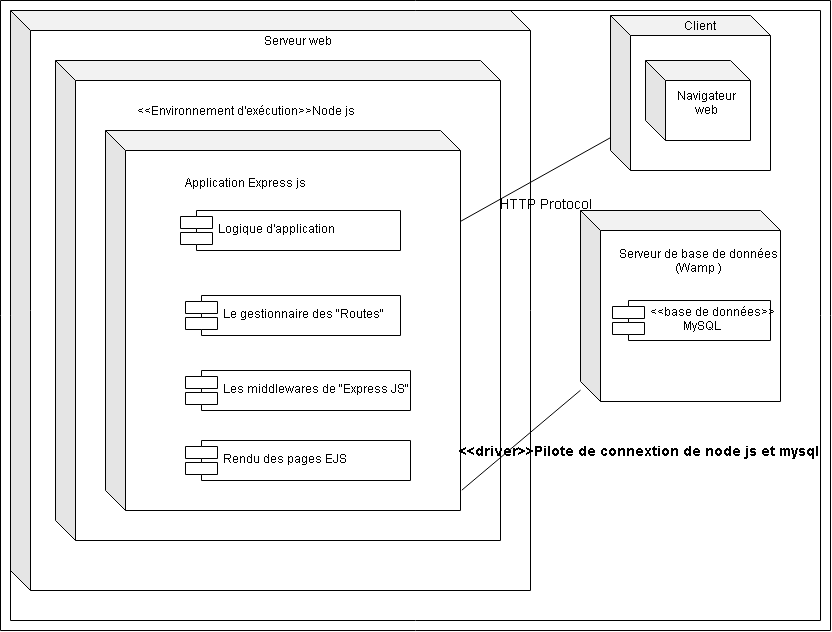
\includegraphics[width=13cm,height=11cm]{./figures/deployement.png}
\caption{Diagramme de d\'{e}ploiement.}
\end{figure}
\FloatBarrier


\section{Diagramme d'activit\'{e}}
Le diagramme d'activit\'{e} nous permet de d\'{e}crire les traitements. Il est
particuli\`{e}rement adapt\'{e} \`{a} la mod\'{e}lisation du cheminement de flots de
contr\^{o}le et de flots de donn\'{e}es. Il permet ainsi de repr\'{e}senter le
comportement d'une m\'{e}thode ou le d\'{e}roulement d'un cas d'utilisation dans
un graphe.
Les diagrammes d'activit\'{e}s sont tr\`{e}s proches des diagrammes d'\'{e}tats-
transitions dans leur pr\'{e}sentation, mais leur interpr\'{e}tation est diff\'{e}rente.
Une activit\'{e} repr\'{e}sente une ex\'{e}cution d'un m\'{e}canisme, un d\'{e}roulement
d'\'{e}tapes s\'{e}quentielles. Le passage d'une activit\'{e} vers une autre est mat\'{e}rialis\'{e}
par une transition.
Les transitions sont d\'{e}clench\'{e}es par la fin d'une activit\'{e} et provoquent le
d\'{e}but imm\'{e}diat d'une autre.
Dans la page suivante , nous pr\'{e}sentons notre diagramme d'activit\'{e} qui illustre le
d\'{e}roulement s\'{e}quentiel des traitements accomplis par l'administrateur afin de
cr\'{e}er et g\'{e}rer un projet.
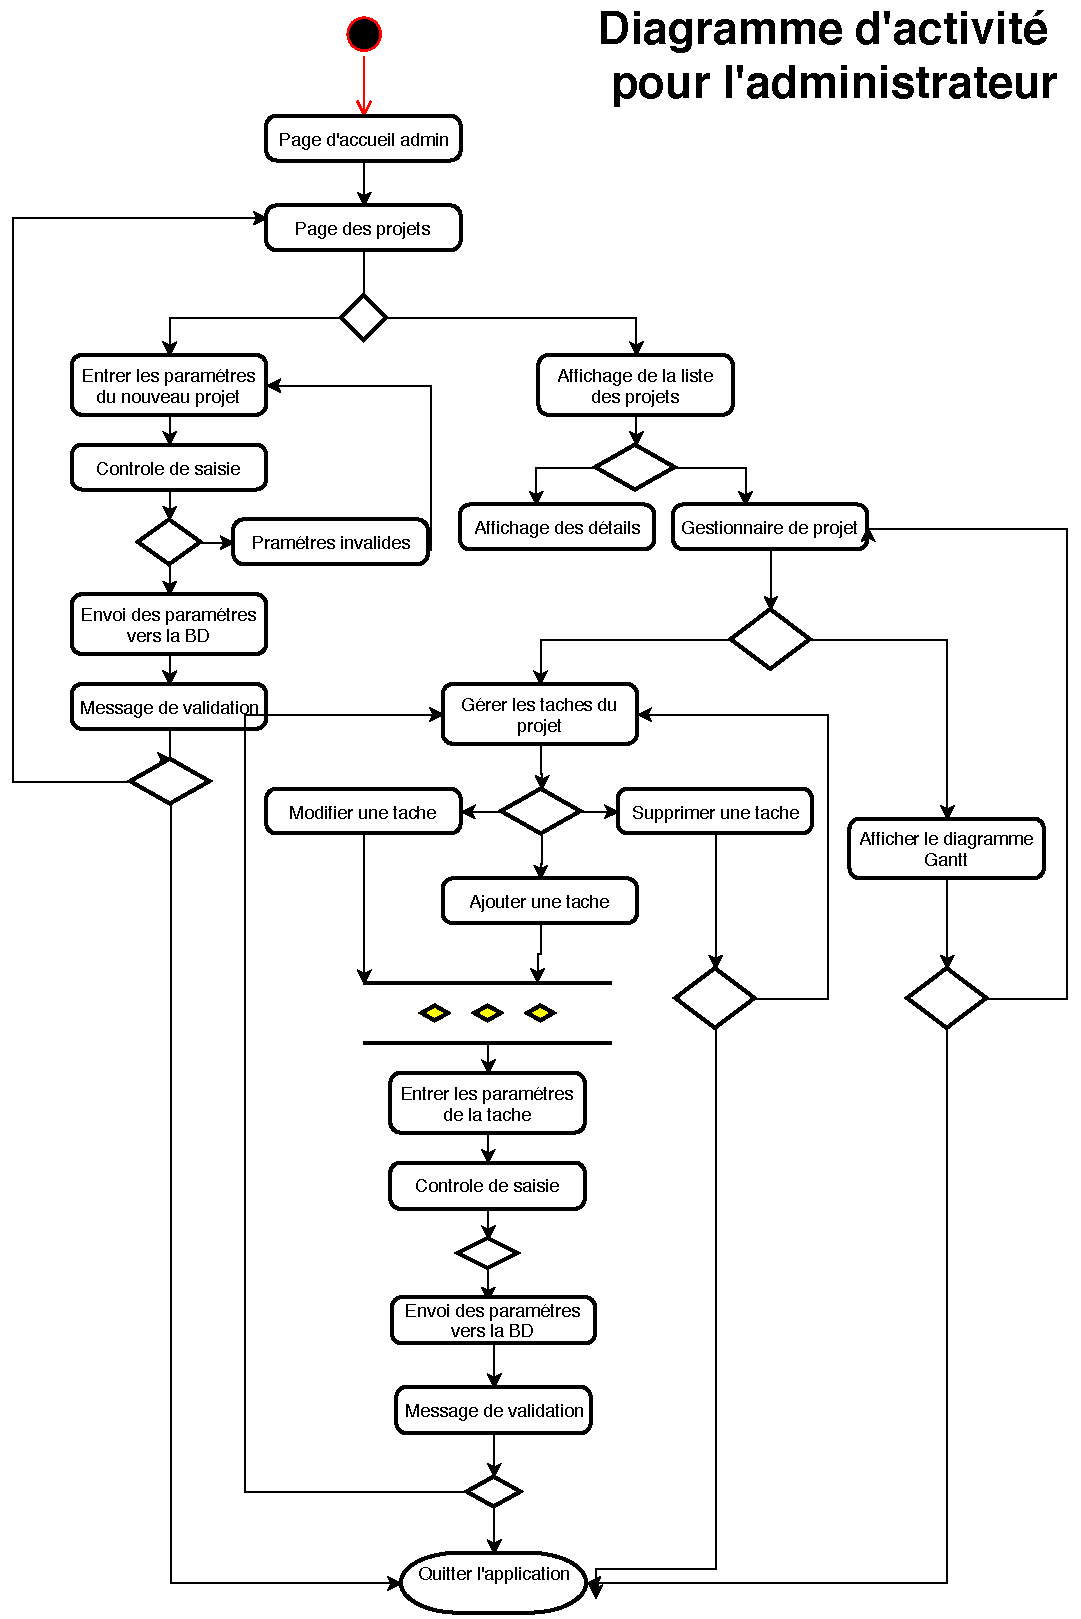
\includepdf{./pdf/activity.pdf}


Ainsi , la figure suivante représente le diagramme d'activit\'{e} pour un membre :
\begin{figure}[H]
\center
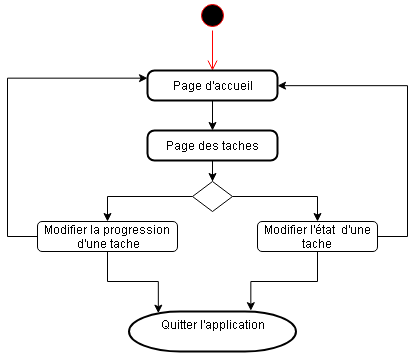
\includegraphics[width=13cm,height=11cm]{./figures/activity_m.png}
\caption{Diagramme d'activit\'{e} pour un membre.}

\end{figure}
\FloatBarrier
